\section{Comparison of kinematic quantities with full simulation}
\label{sec:cmsdelphescomp}
We compare the important kinematic variables used for the study with the CMSSW full
simulation using the LM1 benchmark point. Figures~\ref{fig:njetht},~\ref{fig:jetpteta},~\ref{fig:alphat}
show that the simulation using our {\tt Delphes}-based infrastructure agree well with the full simulation.

\begin{figure}[htbp]
\begin{center}
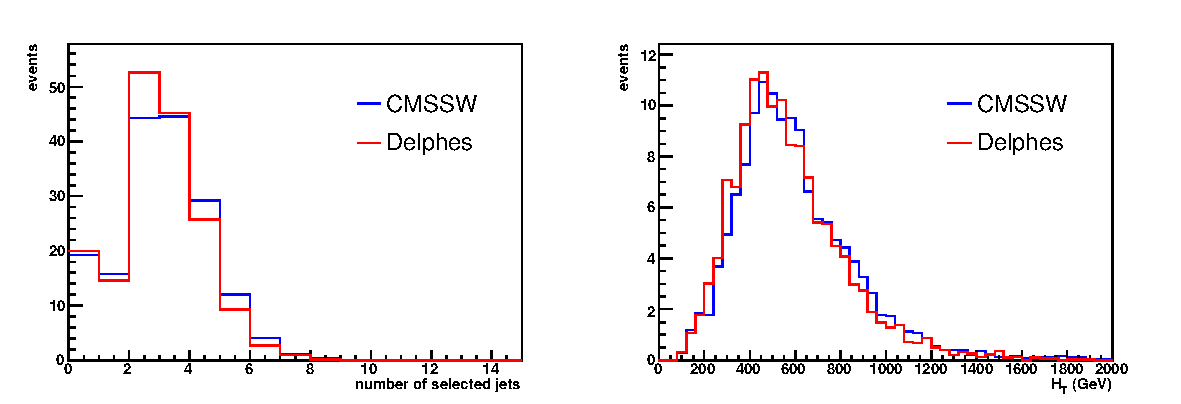
\includegraphics[height=5.5cm]{figs/njetht.pdf} 
\caption{Distributions using the CMSSW full simulation and {\tt Delphes} for the LM1 benchmark point as a function of jet multiplicity (left) and $H_T$ (right)}.
\label{fig:njetht}
\end{center}
\end{figure}


\begin{figure}[htbp]
\begin{center}
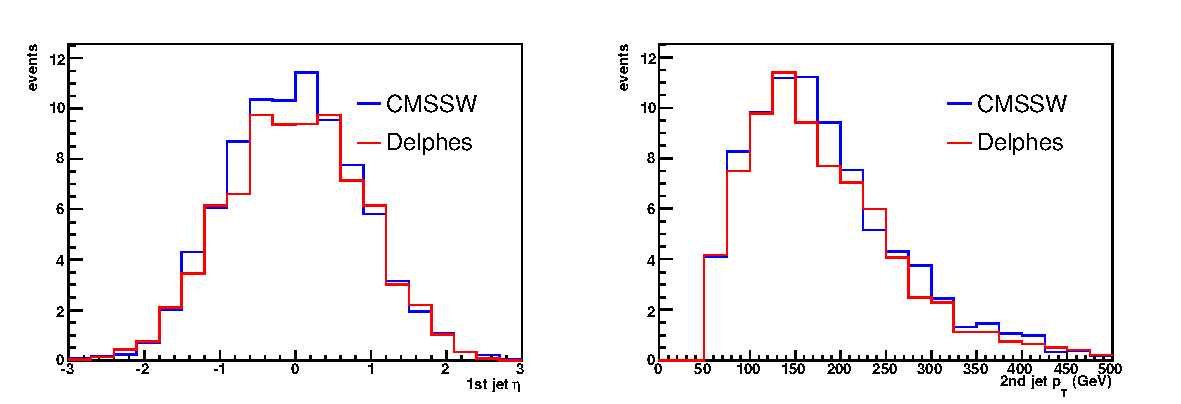
\includegraphics[height=5.5cm]{figs/jet1pteta.pdf} 
\caption{Distributions using the CMSSW full simulation and {\tt Delphes} for the LM1 benchmark point 
as a function of jet pseudorapidity (left) and $p_T$ (right)}.
\label{fig:jetpteta}
\end{center}
\end{figure}

\begin{figure}[htbp]
\begin{center}
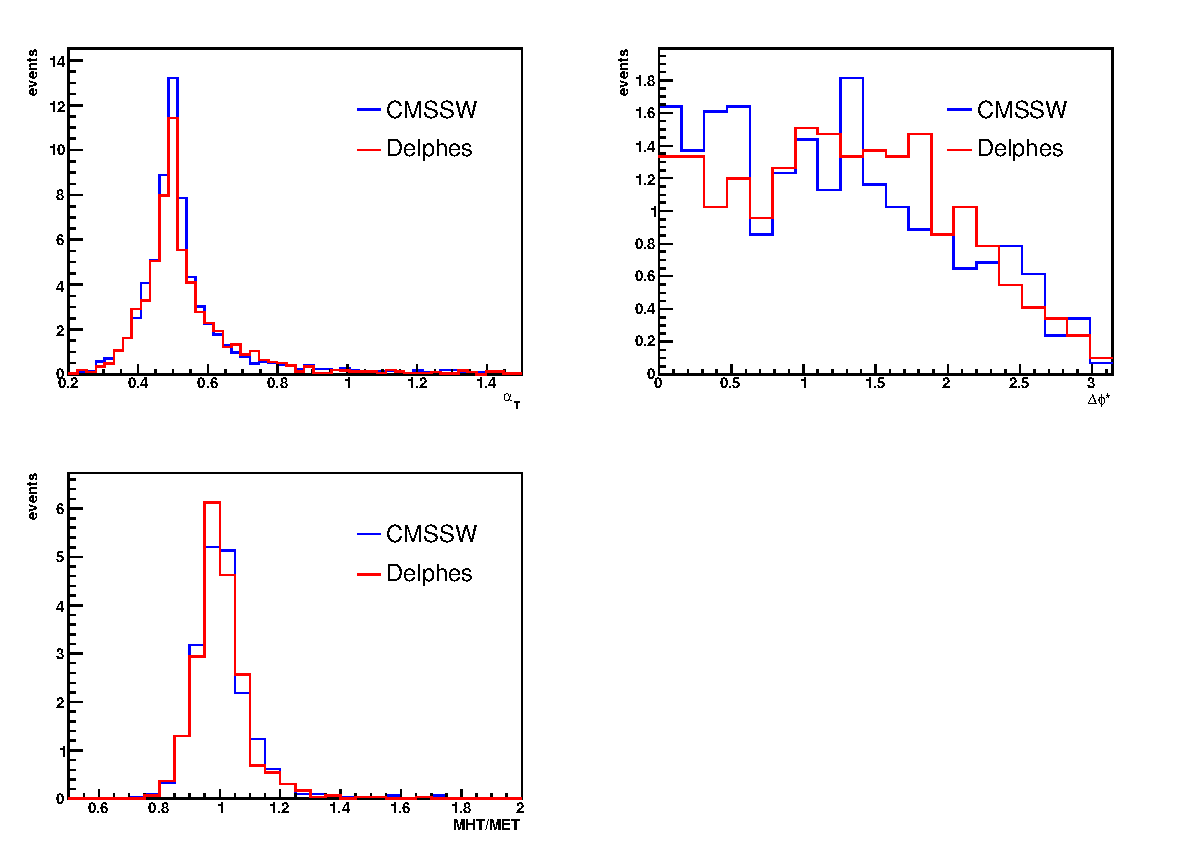
\includegraphics[height=9.cm]{figs/alphat.pdf} 
\caption{Distributions using the CMSSW full simulation and {\tt Delphes} for the LM1 benchmark point
as a function of $\alpha_{T}$ (top left), $\Delta \phi^{*}$ (top right) and MHT/MET (bottom)}.
\label{fig:alphat}
\end{center}
\end{figure}

